\documentclass[uplatex,a4paper,11pt,dvipdfmx]{jsarticle}


% 数式
\usepackage{amsthm}
\usepackage{amsmath,amsfonts,amssymb}
\usepackage{color}
\usepackage{comment}
\usepackage{ulem}
\usepackage[all]{xy}
\usepackage{tikz-cd}
\usepackage{mathtools}
\def\objectstyle{\displaystyle}




\newtheoremstyle{mystyle}% % スタイル名
 {}% % 上部スペース
 {}% % 下部スペース
 {\normalfont}% % 本文フォント
 {}% % インデント量
 {\bf}% % 見出しフォント
 {}% % 見出し後の句読点, '.'
 { }% % 見出し後のスペース, ' ' or \newline
 {\underline{\thmname{#1}\thmnumber{#2}\thmnote{(#3)}}}%
 % 見出しの書式 (can be left empty, meaning `normal')
\theoremstyle{mystyle} % スタイルの適用

\newtheorem{theorem}{Thm.}[section]
\newtheorem{proposition}[theorem]{Prop.}
\newtheorem{lemma}[theorem]{Lem.}
\newtheorem{corollary}[theorem]{Cor.}
\newtheorem{fact}[theorem]{Fact.}
\newtheorem{example}[theorem]{Ex.}

\makeatletter % use at mark
\renewenvironment{proof}[1][\proofname]{\par
 \pushQED{\qed}%
 \normalfont \topsep6\p@\@plus6\p@\relax
 \trivlist
 \item[\hskip\labelsep
 \itshape
 {\bf\underline{#1}}]\ignorespaces
 % {\bf\underline{#1}\@addpunct{.}}]\ignorespaces % ピリオドあり
}{%
 \popQED\endtrivlist\@endpefalse
}
\makeatother % end at mark

\renewcommand{\abstractname}{}
\renewcommand{\theenumi}{(\arabic{enumi})}
\renewcommand{\labelenumi}{(\arabic{enumi})}
\newenvironment{sumipmatrix}{\left ( \begin{smallmatrix}} {\end{smallmatrix}\right )}

\newcommand{\emphasis}[1]{\textgt{\textcolor{magenta}{#1}}}
\DeclareMathOperator{\Aut}{Aut}
\DeclareMathOperator{\Spec}{Spec}
\DeclareMathOperator{\Auteq}{Auteq}\DeclareMathOperator{\Coh}{Coh}
\DeclareMathOperator{\Hom}{Hom}
\DeclareMathOperator{\Ext}{Ext}
\DeclareMathOperator{\Ker}{Ker}
\DeclareMathOperator{\Pic}{Pic}

\DeclareMathOperator{\id}{id}
\DeclareMathOperator{\ch}{ch}
\DeclareMathOperator{\td}{td}
\DeclareMathOperator{\codim}{codim}
\DeclareMathOperator{\Cone}{Cone}
\DeclareMathOperator{\MCG}{MCG}
\DeclareMathOperator{\PMCG}{PMCG}
\DeclareMathOperator{\Out}{Out}
\newcommand{\Extsheaf}{\mathop{\mathcal{E}\! \mathit{xt}}\nolimits}
\newcommand{\Torsheaf}{\mathop{\mathcal{T}\! \mathit{or}}\nolimits}



\begin{document}

\title{}
\author{}
\date{}
%\maketitle
\section{自己同値の誘導}
elliptic surface $\pi \colon S \to C$の定義などは\cite{Ueh15}に従う.
\begin{theorem}
	$\pi \colon S \to C$をelliptic surfaceとし,$G \subset S$を$(-2)$-curve,$a \in \mathbb{Z}$を整数とする.このとき$S$のspherical object $\mathcal{O}_G(a)$に付随するtwist functorの核$$P = \Cone(\mathcal{O}_G(a) \boxtimes \mathcal{O}_G(a)^\vee \xrightarrow{ev} \mathcal{O}_\Delta)$$は$S\times_C S$上の層である.
\end{theorem}
\begin{lemma}\label{flatness}
	$\pi \colon S \to C$をelliptic surfaceとする.この時$\pi$はflatである.
\end{lemma}
\begin{proof}
	$\pi(x)=y$とおくと,局所環の射$\mathcal{O}_{C, y} \to \mathcal{O}_{S, x}$が誘導される.$\mathcal{O}_{C, y} $はPIDで,$\mathcal{O}_{S, x}$は正則局所環だから特に整域である.よって$\mathcal{O}_{S, x}$はPID上のtorsion-free加群だからflatである.
\end{proof}
\begin{lemma}\label{Cartesian}
	図式
	\[
		\xymatrix{
			S \times_C S \ar[r] \ar[d]& S \times S \ar[d]^{\pi \times \pi}\\
			C \ar[r]^{\Delta_C} & C \times C
		}
	\]
	はカルテシアンである.
\end{lemma}
\begin{proof}
	いわゆるmagic diagram.
\end{proof}
\begin{lemma}\label{effective_divisor}
	$X = S \times_C S, Y = S \times S$とし,$i \colon X \to Y$をinclusionとする.このとき$Y$上のline bundle $L$ と完全列$$0 \to L \to \mathcal{O}_Y \to \mathcal{O}_X \to 0$$がある.ここで$\mathcal{O}_Y \to \mathcal{O}_X$は自然な全射である.
\end{lemma}
\begin{proof}
	$C$は非特異だから,$\Delta_C\colon C \to C \times C$により$C$は$C\times C$の中でlocal complete intersectionであり,完全列$$0 \to \mathcal{O}_{C\times C}(-\Delta) \to \mathcal{O}_{C \times C} \to \mathcal{O}_{\Delta} \to 0$$がある.さらにLem.\ref{flatness}より$\pi \times \pi$はflatだから,この完全列を$\pi \times \pi$でpullbackしてLem.\ref{Cartesian}の図式と組み合わせると求める完全列を得る.
\end{proof}
\begin{comment}
\begin{lemma}
	$Y$を非特異代数多様体とし,$X \subset Y$をregular immersionとする.また$C_{X/Y}$をそのconormal sheafとする.このとき任意の$F \in \Coh(X)$について$$Li^*(i_*F) \cong \bigoplus_{k = 0}^r (F\otimes \wedge^k C_{X/Y})[k]$$となる.
\end{lemma}
\begin{proof}
	$i_* \colon D^*(X) \to D^*(Y)$はexactだから$i_*Li^* \cong L(i_*i^*)$である.ここで$i_*i^* \cong -\otimes_{\mathcal{O}_Y}\mathcal{O}_X$だから,$L(i_*i^*) \cong -\otimes^L_{\mathcal{O}_Y}\mathcal{O}_X$となる.またregular immersionの仮定より,Koszul resolution
\end{proof}
\end{comment}
\begin{lemma}\label{counit_map}
	Lem.\ref{effective_divisor}の状況で$F \in \Coh(X)$とすると,随伴$Li^* \dashv i_*$に付随するcounit射$\varepsilon \colon Li^*(i_*F) \to F$が複体の$0$次コホモロジーに誘導する射は同型である.
\end{lemma}
\begin{proof}
	$i_*F \in \Coh(Y)$の bounded locally free resolution
	$$0 \to P^{-r}\to\cdots\to P^{-1}\to P^0 \to i_* F \to 0$$
	をとる.これにより得られる$D^b(Y)$での同型射を$\varphi \colon P^\bullet \to i_*F$とする.随伴の自然性より以下のような可換図式がある.
	\[
		\begin{tikzcd}
			\Hom_Y(i_*F, i_*F) \arrow[r, "\sim"]\arrow[d, "- \circ \varphi"] & \Hom_X(Li^*(i_*F), F) \arrow[d, "- \circ Li^*(\varphi)"]&\id \arrow[r, mapsto]\arrow[d, mapsto] & \varepsilon \arrow[d, mapsto]\\
			\Hom_Y(P^\bullet, i_*F) \arrow[r, "\sim"] & \Hom_X(Li^*(P^\bullet), F)&\varphi \arrow[r, mapsto] & \varepsilon \circ Li^*(\varphi)
		\end{tikzcd}
	\]
	$\varepsilon$の代わりに$\varepsilon \circ Li^*(\varphi)$が$0$次コホモロジー誘導する射について確かめればよい.上の可換図式より,$\varepsilon \circ Li^*(\varphi)$は$\varphi$を随伴でうつしたもの等しいが,下の段の随伴同型は derived でない随伴同型による複体の射の対応(から誘導されるもの)である.よって以下の$\varphi$
	\[
		\begin{tikzcd}
			\cdots\to &P^{-1}\arrow[d]&\to &P^0 \arrow[d, "\varphi^0"] &\to &0\arrow[d]\\
			&0&\to& i_*F & \to &0
		\end{tikzcd}
	\]
	を随伴でうつしたものは,$\varphi^0$を随伴でうつした$\psi^0$を用いて
	\[
		\begin{tikzcd}
			\cdots\to &i^*P^{-1}\arrow[d]&\to &i^*P^0 \arrow[d, "\psi^0"] &\to &0\arrow[d]\\
			&0&\to& F & \to &0
		\end{tikzcd}
	\]
	と表される射$\psi$である.derived でない順像逆像随伴の構成より,$\psi^0$は$\varphi^0$の$X$への制限に等しいから,$i^*$の右完全性より$0$次のコホモロジーに誘導する射は同型である.


\end{proof}



\begin{lemma}\label{pullback}
	Lem.\ref{effective_divisor}の状況で$F \in \Coh(X)$とすると$D^b(X)$におけるdistinguished triangle
	$$(F\otimes L_{|X})[1] \to Li^*(i_*F) \to F \xrightarrow{+1}$$がある.さらにこの図式の$Li^*(i_*F) \to F$は,随伴$Li^* \dashv i_*$に付随するcounit射$\varepsilon \colon Li^*(i_*F) \to F$である.
\end{lemma}
\begin{proof}
	$i_* \colon D^*(X) \to D^*(Y)$はexactだから$i_*Li^* \cong L(i_*i^*)$である.ここで$i_*i^* \cong -\otimes_{\mathcal{O}_Y}\mathcal{O}_X$だから,$L(i_*i^*) \cong -\otimes^L_{\mathcal{O}_Y}\mathcal{O}_X$となる.よってLem.\ref{effective_divisor}の完全列により$\mathcal{O}_X$を分解することで$$L(i_*i^*)(i_*F) \cong (\cdots \to 0 \to i_*F\otimes L \xrightarrow{d^{-1}} i_*F \to 0 \to \cdots)$$となる($i_*F$が$0$次のcomplex).このとき,$d^{-1}$が$0$射であることをしめす.問題はlocalなので$X, Y$はaffineとしてよい.$Y=\Spec{A}, X = \Spec{A/I}$とし,$F$は$A/I$加群$M$に付随する層だとする.Lem.\ref{effective_divisor}の完全列は$$0 \to A \to A \to A/I \to 0$$となり,左の射は$I$の生成元$f$による$f$倍写像である.すると$d^{-1}$は$f$倍写像$M \to M$となるが,$M$は$A/I$加群なのでこれは$0$射に等しい.

	ここまでで$$i_*Li^*(i_*F) \cong i_*F[0] \oplus i_*(F\otimes L)[1]$$が示せた.さらに$i_*$は完全関手だからコホモロジーをとる操作と可換であることに注意すると,複体$Li^*(i_*F)$の$j$次コホモロジー$\mathcal{H}^j$について$$i_*\mathcal{H}^0 \cong i_*F$$$$i_*\mathcal{H}^{-1}\cong i_*(F \otimes L_{|X})$$$$i_*\mathcal{H}^j = 0 \hspace{10pt}(j \neq 0, -1)$$となる.よって$$\mathcal{H}^0 \cong F$$$$\mathcal{H}^{-1}\cong F \otimes L_{|X}$$$$\mathcal{H}^j = 0 \hspace{10pt}(j \neq 0, -1)$$となる.ここでcounit射$\varepsilon \colon Li^*(i_*F) \to F$を補完するようなdistinguished triangle$$C\to Li^*(i_*F) \xrightarrow{\varepsilon} F \xrightarrow{+1}$$をとる.これに付随するコホモロジー長完全列をとると

	\[
		\begin{array}{ccccccc}
			 &     &                     &     & \cdots           & \to                                      & 0 \\
			 & \to & \mathcal{H}^{-2}(C) & \to & 0                & \to                                      & 0 \\
			 & \to & \mathcal{H}^{-1}(C) & \to & F \otimes L_{|X} & \to                                      & 0 \\
			 & \to & \mathcal{H}^{0}(C)  & \to & F                & \xrightarrow{\mathcal{H}^0(\varepsilon)} & F \\
			 & \to & \mathcal{H}^{1}(C)  & \to & 0                & \to                                      & 0 \\
			 & \to & \cdots              &     &                  &                                          &   \\
		\end{array}
	\]
	となり,Lem.\ref{counit_map}より$\mathcal{H}^0(\varepsilon)$は同型だから,$C \cong (F \otimes L_{|X})[1]$となる.
\end{proof}
\begin{lemma}\label{boxtimes_is_a_sheaf}
	$G \subset S$が$(-2)$-curveで$a \in \mathbb{Z}$とする.以下のいずれかを仮定する.
	\begin{itemize}
		\item $\pi \colon S \to C$はsectionをもつ.
		\item $\pi \colon S \to C$のsingular fiber $E$は$I_n$型$n \geq 3$である.
	\end{itemize}
	このとき,$\mathcal{O}_G(a)^\vee \boxtimes \mathcal{O}_G(a) \in D^b(S\times S)$は$G\times G$上の層の$-1$シフト(のpushforward)である.
\end{lemma}
\begin{proof}
	$S$上のdivisor $D$であって$G.D = a$であるものを1つとる(sectionを持つときはsectionの$a$倍,$N \geq 3$の$I_n$型のときは$G$のとなりの既約成分の$a$倍をとればよい).このとき$\mathcal{O}_S(D)_{|G} \cong \mathcal{O}_G(a)$である.完全列$$0 \to \mathcal{O}_S(-G) \to \mathcal{O}_S \to \mathcal{O}_G \to 0$$より,$D^b(S)$において$$\mathcal{O}_G(a) \cong (\cdots \to 0 \to \mathcal{O}_S(D-G) \to \mathcal{O}_S(D) \to 0 \to \cdots)$$となる(右辺は$0$次に$\mathcal{O}_S(D)$があるcomplex).よって
	\begin{align*}
		\mathcal{O}_G(a)^\vee & \cong (\cdots \to 0 \to \mathcal{O}_S(-D) \to \mathcal{O}_S(G-D) \to 0 \to \cdots) \\
		                      & \cong \mathcal{O}_S(G-D)_{|G}[-1]
	\end{align*}
	となる.すると
	\begin{align*}
		 & \mathcal{O}_G(a)^\vee \boxtimes \mathcal{O}_G(a)                                                                                 \\
		 & \cong p_1^*\mathcal{O}_S(G-D)_{|G} \otimes^L p_2^*\mathcal{O}_S(D)_{|G}[-1]                                                      \\
		 & \cong \mathcal{O}_{S\times S}(G\times S - D\times S)_{|G\times S} \otimes^L \mathcal{O}_{S\times S}(S \times D)_{|S\times G}[-1] \\
	\end{align*}
	となる.よってderived tensorのhigher cohomologyが消えていることを示せばこれは
	\begin{align*}
		 & \mathcal{O}_{S\times S}(G\times S - D\times S)_{|G\times S} \otimes \mathcal{O}_{S\times S}(S \times D)_{|S\times G}[-1] \\
		 & = \mathcal{O}_{S\times S}(G\times S - D\times S+S \times D)_{|G\times G}[-1]
	\end{align*}
	となり命題が示される.問題はlocalなので$\mathcal{O}_{S\times S}(D\times S)_{|G\times S - D\times S}$と$\mathcal{O}_{S\times S}(S \times D)_{|S\times G}$はそれぞれ$\mathcal{O}_{G\times S}$と$\mathcal{O}_{S\times G}$だと思ってよく,すると$G \times S$と$S \times G$が$S \times S$の中でtransversal intersectionなので全ての$q>0$について$$\Torsheaf_q^{\mathcal{O}_{S\times S}}(\mathcal{O}_{G\times S}, \mathcal{O}_{S\times G})=0$$となりderived tensorのhigher cohomologyが消えていることがわかる.
\end{proof}
\begin{theorem}
	$\pi \colon S \to C$をelliptic surfaceとし,$G \subset S$を$(-2)$-curve,$a \in \mathbb{Z}$を整数とする.このとき$S$のspherical object $\mathcal{O}_G(a)$に付随するtwist functorの核$$P = \Cone(\mathcal{O}_G(a)^\vee \boxtimes \mathcal{O}_G(a) \xrightarrow{ev} \mathcal{O}_\Delta)$$は$S\times_C S$上のcomplex(より強く,層)のpushforwardである.
\end{theorem}
\begin{proof}
	Lem.\ref{boxtimes_is_a_sheaf}より,$G\times G$上の層$F$を用いて$\mathcal{O}_G(a)^\vee \boxtimes \mathcal{O}_G(a)\cong F[-1]$と表せる.よって$D^b(S \times S)$におけるdistinguished triangle$$F[-1] \xrightarrow{ev} \mathcal{O}_\Delta \to P \xrightarrow{+1} F$$がある.ここでもし$ev \in \Hom_{D^b(S\times S)}(F[-1], \mathcal{O}_\Delta)$が$\Hom_{D^b(S\times_C S)}(F[-1], \mathcal{O}_\Delta)$の元の像だったとすると,$D^b(S\times_C S)$でのCone$$P' = \Cone(\mathcal{O}_G(a)^\vee \boxtimes \mathcal{O}_G(a) \xrightarrow{ev} \mathcal{O}_\Delta)$$を$D^b(S\times S)$にpushしたものは$P$と同型になる.よってinclusion $S\times_C S \to S\times S$による(derived)pushforwardが誘導する射$$\Hom_{D^b(S\times_C S)}(F[-1], \mathcal{O}_\Delta) \to \Hom_{D^b(S\times S)}(F[-1], \mathcal{O}_\Delta)$$が全射であることを証明すれば定理が示される.

	以下$X=S\times_C S$,$ Y=S\times S$とおき,$i \colon X \to Y$を自然なinclusionとする.
	Lem.\ref{pullback}の distinguished triangle に $R\Hom(-, \mathcal{O}_\Delta)$をあてると
	$$R\Hom(F, \mathcal{O}_\Delta) \to R\Hom(Li^*(i_*F), \mathcal{O}_\Delta) \to R\Hom((F\otimes L_{|X})[1], \mathcal{O}_\Delta) \xrightarrow{+1}$$
	となり,コホモロジー長完全列をとることで
	\[
		\begin{array}{ccccccc}
			 &     &                               &     &                                        &     & 0                                         \\
			 & \to & \Ext^1(F, \mathcal{O}_\Delta) & \to & \Ext^1(Li^*(i_*F), \mathcal{O}_\Delta) & \to & \Hom(F\otimes L_{|X}, \mathcal{O}_\Delta) \\
			 & \to & \Ext^2(F, \mathcal{O}_\Delta) & \to & \cdots                                 &     &
		\end{array}
	\]
	という完全列を得る.この図式における$$\Ext^1(F, \mathcal{O}_\Delta) \to \Ext^1(Li^*(i_*F), \mathcal{O}_\Delta)$$はLem.\ref{pullback}より随伴$Li^* \dashv i_*$に付随するcounit射$\varepsilon \colon Li^*(i_*F) \to F$から誘導されるものだから,随伴同型$\Ext_Y^1(i_*F, i_*\mathcal{O}_\Delta) \cong \Ext_X^1(Li^*(i_*F), \mathcal{O}_\Delta)$によりpushforwardが誘導する射$$\Ext_X^1(F, \mathcal{O}_\Delta) \to \Ext_Y^1(i_*F, i_*\mathcal{O}_\Delta)$$と同一視される.よって上の長完全列より,$\Hom(F\otimes L_{|X}, \mathcal{O}_\Delta) =0$であることを証明すれば命題が示されることになる.

	以下それを示す.随伴により$$\Hom_X(F\otimes L_{|X}, \mathcal{O}_\Delta)\cong\Hom_\Delta((F\otimes L_{|X})_{|\Delta}, \mathcal{O}_\Delta)$$だが,$F$は$G \times G \subset X$上の層だったため,$(F\otimes L_{|X})_{|\Delta}$は$(G \times G) \cap \Delta = \Delta_G$上の層$F'$である.よって$$\Hom_\Delta((F\otimes L_{|X})_{|\Delta}, \mathcal{O}_\Delta)=\Hom_\Delta(F', \mathcal{O}_\Delta)$$となり,$\Delta_G \subset \Delta$は$G \subset S$とみなせるため,結局$G$上の層$F'$について$\Hom_S(F', \mathcal{O}_S)=0$を証明すればよい.これはSerre dualityより明らか.
\end{proof}

\begin{corollary}\label{restriction_map}
	$B = \langle T_{\mathcal{O}_G(a)} \mid G \colon \text{$(-2)$-curve}, a \in \mathbb{Z} \rangle \subset \Auteq D^b(S)$の元は積分核の$E\times E$への制限によって$D^b(E)$の自己同値を誘導し,それによる写像$$r \colon B \to \Auteq D^b(E)$$は群準同型である.さらに$i \colon E \hookrightarrow S$とおくと,任意の$\Phi \in B$について関手の同型$$\Phi \circ i_* \cong i_* \circ r(\Phi)$$が成り立つ.
\end{corollary}
\begin{proof}
	積分関手$\Phi_P, \Phi_Q \colon D^b(S) \to D^b(S)$の核$P, Q$がともに$S \times_C S$上のcomplexのpushforwardならば,その合成$\Phi_Q \circ \Phi_P$の核も$S \times_C S$上のcomplexのpushforwardである.よって写像$r$が定まる.群準同型であることはflat base change formulaからわかる.最後の部分も同様.
\end{proof}
\begin{proposition}
	$E$を$I_n$型とし$E = \bigcup_{i=1}^n G_i$と既約成分分解すると,$$\Ker r = \{-\otimes \mathcal{O}(aE) \mid a \in \mathbb{Z}\} \cong \mathbb{Z}$$である.
\end{proposition}
\begin{proof}
	$\Phi \in B$とし,$r(\Phi) = \id$だとする.このときCor.\ref{restriction_map}の同型$$\Phi \circ i_* \cong i_* \circ r(\Phi)$$より,任意の閉点$x \in E$について$\Phi(\mathcal{O}_x) \cong \mathcal{O}_x$である.また$E$の外では$T_{\mathcal{O}_G(a)}$の核が$\mathcal{O}_\Delta$に等しいことから,$x \in S\setminus E$について$T_{\mathcal{O}_G(a)}(\mathcal{O}_x) \cong \mathcal{O}_x$となり,その合成である$\Phi$についても$\Phi(\mathcal{O}_x) \cong\mathcal{O}_x$となる.よって\cite{Huy06} Cor.5.23 より,ある直線束$L \in \Pic(S)$により$$\Phi \cong (-)\otimes L$$とかける.ここで\cite{IU05} Prop.4.18 と同様にして$$B \cap \Pic(S) = \{ (-)\otimes \mathcal{O}(\sum_{i=1}^n a_iG_i) \mid a_i \in \mathbb{Z}\}$$となるから,$$\Phi \cong (-)\otimes \mathcal{O}(\sum_{i=1}^n a_iG_i)$$とかける.よって$r(\Phi) \cong (-)\otimes \mathcal{O}(\sum_{i=1}^n a_iG_i)|_E$となり,これが$\id$になるためには(各$G_i$での次数を見ることで)$$a_{i-1} - 2a_i + a_{i+1} = 0, \hspace{10pt} (i = 1, 2, \dots, n)$$が必要となる.(ただし$a_0 \coloneqq a_n, a_{n+1} \coloneqq a_1$とする.)よって全ての$a_i$が等しいことが必要だから$\Phi \colon (-)\otimes \mathcal{O}(aE)$とかけて,逆にこのとき$r(\Phi) \cong \id$である.
\end{proof}

\section{誘導される自己同値の計算}
\subsection{Chern classとRHomの計算}
\begin{proposition}
	$S$上のsheafと見たときに
	\begin{enumerate}
		\item $c_1(\mathcal{O}_G) = G, c_2(\mathcal{O}_G) = -2, \ch(\mathcal{O}_G) = (0, G, 1)$

		\item $c_1(\mathcal{O}_x) = 0, c_2(\mathcal{O}_x) = -1, \ch(\mathcal{O}_x) = (0, 0, 1)$
		\item $c_1(\mathcal{O}_G(-1)) = G, c_2(\mathcal{O}_G(-1)) = -1, \ch(\mathcal{O}_G(-1)) = (0, G, 0)$
		\item $c_1(\mathcal{O}_E) = E, c_2(\mathcal{O}_E) = 0, \ch(\mathcal{O}_E) = (0, E, 1)$
	\end{enumerate}
\end{proposition}
\begin{proof}
	\begin{enumerate}
		\item 完全列$$0 \to \mathcal{O}_S(-G) \to \mathcal{O}_S \to \mathcal{O}_G \to 0$$のtotal Chern classをとると$$1 = c(\mathcal{O}_S) = c(\mathcal{O}_S(-G))c(\mathcal{O}_G)$$で,$c(\mathcal{O}_S(-G)) = 1-G$だから$$c(\mathcal{O}_G) = \frac{1}{1-G} = 1+G+G^2$$これと$G^2=-2$よりよい.

		\item Grothendieck-Riemann-Rochより$\ch(\mathcal{O}_x)\td(S) = (0, 0, 1)$である.これと$\td(S) = (1, -K_S/2, \chi(\mathcal{O}_S))$からわかる.
		\item 完全列$$0 \to \mathcal{O}_G(-1) \to \mathcal{O}_G \to \mathcal{O}_x \to 0$$より$$\ch( \mathcal{O}_G(-1)) = \ch(\mathcal{O}_G) - \ch(\mathcal{O}_x) = (0, G, 0)$$である.ここから$c_1(\mathcal{O}_G(-1)) = G, c_2(\mathcal{O}_G(-1)) = -1$もわかる.
	\end{enumerate}
\end{proof}
\begin{proposition}
	$G$と$G'$はとなりあう$E$の既約成分,$x$は$G$上の点とする.
	\begin{enumerate}
		\item $R\Hom_S(\mathcal{O}_G, \mathcal{O}_{G'}) = \mathbb{C}[-1]$
		\item $R\Hom_S(\mathcal{O}_G, \mathcal{O}_E) = \mathbb{C}[-1]\oplus\mathbb{C}[-2]$
		\item $R\Hom_S(\mathcal{O}_G, \mathcal{O}_x) = \mathbb{C}\oplus\mathbb{C}[-1]$
		\item $R\Hom_S(\mathcal{O}_G(-1), \mathcal{O}_{G'}(-1)) = \mathbb{C}[-1]$
		\item $R\Hom_S(\mathcal{O}_G(-1), \mathcal{O}_E) = 0$
		\item $R\Hom_S(\mathcal{O}_G(-1), \mathcal{O}_x) = \mathbb{C}\oplus\mathbb{C}[-1]$
	\end{enumerate}
\end{proposition}
\begin{proof}
	曲面のadjunction formulaより$G.K_S = 0$だから,$\mathcal{O}_G \otimes \omega_S \cong \mathcal{O}_G$となることに注意する.
	\begin{enumerate}
		\item 順像逆像随伴により$$\Hom_S(\mathcal{O}_G, \mathcal{O}_{G'}) = \Hom_{G'}(\mathcal{O}_{G\cap G'}, \mathcal{O}_{G'}) = 0$$である.またと
		      \begin{align*}
			      \Ext_S^2(\mathcal{O}_G, \mathcal{O}_{G'}) & \cong \Hom_S(\mathcal{O}_{G'}, \mathcal{O}_G \otimes \omega_S)^* \\
			                                                & =\Hom_S(\mathcal{O}_{G'}, \mathcal{O}_G \otimes \omega_S)^*      \\
			                                                & =\Hom_S(\mathcal{O}_{G'}, \mathcal{O}_G)^*                       \\
			                                                & =0
		      \end{align*}
		      である.さらにHirzebruch-Riemann-Rochより$\chi(\mathcal{O}_G, \mathcal{O}_{G'}) = -G.G' = -1$だから,$\Ext_S^1(\mathcal{O}_G, \mathcal{O}_{G'}) = \mathbb{C}$である.
		\item まず\begin{align*}
			      \Hom_S(\mathcal{O}_G, \mathcal{O}_E) & =\Hom_E(\mathcal{O}_G, \mathcal{O}_E)          \\
			                                           & \cong \Ext^1_E(\mathcal{O}_E, \mathcal{O}_G)^* \\
			                                           & \cong H^1(\mathcal{O}_G)^*                     \\
			                                           & \cong H^1(\mathcal{O}_{\mathbb{P}^1})^*        \\
			                                           & =0
		      \end{align*}
		      となる.また$\Ext^2_S(\mathcal{O}_G, \mathcal{O}_E)\cong\Hom_S(\mathcal{O}_E, \mathcal{O}_G\otimes \omega_S)^* =\mathbb{C}$であり,
		      $$\chi(\mathcal{O}_G, \mathcal{O}_E) = -G.E = 0$$と合わせると$\Ext^1_S(\mathcal{O}_G, \mathcal{O}_E) = \mathbb{C}$がわかる.
		\item $\Hom_S(\mathcal{O}_G, \mathcal{O}_x) = \mathbb{C}$は明らか.$\Ext^2_S(\mathcal{O}_G, \mathcal{O}_x)\cong \Hom_S(\mathcal{O}_x, \mathcal{O}_G\otimes \omega_S)^*=0$と
		      \begin{align*}
			      \chi(\mathcal{O}_G, \mathcal{O}_x) & =\int_S(0, -G, 1)\cdot(0, 0, 1)\cdot(1, -K_S/2, \chi(\mathcal{O}_S)) \\
			                                         & =\int_S (0, -G, 1)\cdot(0, 0, 1)                                     \\
			                                         & =0
		      \end{align*}
		      より$\Ext^1_S(\mathcal{O}_G, \mathcal{O}_x) = \mathbb{C}$となる.
		\item (1)と同様に$\Hom_S=0, \Ext^2_S = 0$であり,$\chi(\mathcal{O}_G(-1), \mathcal{O}_{G'}(-1)) =-G.G' = -1$だからよい.
		\item (2)と同様に\begin{align*}
			      \Hom_S(\mathcal{O}_G(-1), \mathcal{O}_E) & \cong \Hom_E(\mathcal{O}_G(-1),\mathcal{O}_E)      \\
			                                               & \cong \Ext^1_E(\mathcal{O}_E, \mathcal{O}_G(-1))^* \\
			                                               & \cong H^1(\mathcal{O}_G(-1))^*                     \\
			                                               & \cong H^1(\mathcal{O}_{\mathbb{P}^1}(-1))^*        \\
			                                               & =0
		      \end{align*}
		      \begin{align*}
			      \Ext^2_S(\mathcal{O}_G(-1), \mathcal{O}_E) & \cong \Hom_S(\mathcal{O}_E, \mathcal{O}_G(-1)) \\
			                                                 & =H^0(\mathcal{O}_G(-1))                        \\
			                                                 & =0
		      \end{align*}
		      かつ$\chi(\mathcal{O}_E, \mathcal{O}_G(-1)) = -G.E = 0$となる.
		\item (3)と全く同じ.
	\end{enumerate}
\end{proof}


\begin{proposition}
	$G$と$G'$をとなりあう$E$の既約成分とし,$G$と$G'$の交点であるような特異点を$s$,$s$でない$G$上のもう一方の特異点を$t$とする.また$a, b \in \mathbb{Z}$とする.
	\begin{enumerate}
		\item $R\Hom_E(\mathcal{O}_G(a), \mathcal{O}_{G'}(b)) = \bigoplus_{i=1}^\infty \mathbb{C}[-(2i-1)]$つまり$$\Ext^i_E(\mathcal{O}_G(a), \mathcal{O}_{G'}(b)) = \left \{
			      \begin{array}{ll}
				      0          & (i<0 \text{または $i$ が偶数}) \\
				      \mathbb{C} & (\text{ $i$ が正の奇数})
			      \end{array}
			      \right.$$
		\item $R\Hom_E(\mathcal{O}_G(a), \mathcal{O}_G(b)) = H^0(\mathcal{O}_G(b-a)) \oplus \bigoplus_{i=1}^\infty \mathbb{C}[-2i]$つまり$$\Ext^i_E(\mathcal{O}_G(a), \mathcal{O}_G(b)) =\left \{
			      \begin{array}{ll}
				      H^0(\mathcal{O}_G(b-a)) & (i=0)                            \\
				      0                       & (i < 0 \text{または $i$ が奇数}) \\
				      \mathbb{C}^2            & (\text{ $i$ が正の偶数})
			      \end{array}
			      \right.$$
		\item $R\Hom_E(\mathcal{O}_G(a), \mathcal{O}_s) = \bigoplus_{i=0}^\infty \mathbb{C}[-i]$つまり$$\Ext^i_E(\mathcal{O}_G(a), \mathcal{O}_s) =\left \{
			      \begin{array}{ll}
				      0          & (i< 0)    \\
				      \mathbb{C} & (i\geq 0)
			      \end{array}
			      \right.$$
		\item $R\Hom_E(\mathcal{O}_s, \mathcal{O}_G(a)) = \bigoplus_{i=1}^\infty \mathbb{C}[-i]$つまり$$\Ext^i_E(\mathcal{O}_s, \mathcal{O}_G(a)) =\left \{
			      \begin{array}{ll}
				      0          & (i\leq 0) \\
				      \mathbb{C} & (i>0)
			      \end{array}
			      \right.$$
	\end{enumerate}
\end{proposition}
\begin{proof}
	\begin{enumerate}
		\item local-to-global spectral sequenceより,$$\Extsheaf^i_E(\mathcal{O}_G(a), \mathcal{O}_{G'}(b)) = \left \{
			      \begin{array}{ll}
				      0             & (i<0 \text{または $i$ が偶数}) \\
				      \mathcal{O}_s & (\text{ $ i $ が正の奇数})
			      \end{array}
			      \right.$$を示せば十分である.左辺のsupportは$s$だから$s$でのstalkを計算すればよく,特に$a=b=0$としてよい.そこで$s$の周りの$E$の座標として$E = \Spec \mathbb{C}[x,y]/(xy), G = \{x = 0\}, G'=\{y=0\}, s = (0, 0)$となるようなものをとれば,$A=(\mathbb{C}[x,y]/(xy))_{(x,y)}$として$$\Extsheaf^i_E(\mathcal{O}_G, \mathcal{O}_{G'})_s \cong \Ext^i_A(A/x, A/y)$$を計算すればよいことになる.$A/x$の射影分解$$\cdots\to A \xrightarrow{y}A \xrightarrow{x} A \to A/x\to 0$$により$\Ext^i_A(A/x, A/y)$は複体$$0 \to A/y \xrightarrow{x} A/y \xrightarrow{y} A/y \to \cdots$$の$i$次コホモロジーだから,$$ \Ext^i_A(A/x, A/y) = \left \{
			      \begin{array}{ll}
				      0          & (i<0 \text{または $i$ が偶数}) \\
				      \mathbb{C} & (\text{ $ i $ が正の奇数})
			      \end{array}
			      \right.$$となる.
		\item $i=0$については明らかなので,以下$i>0$とする.まず$x \in E\setminus\{s, t\}$について,$$\Extsheaf^i_E(\mathcal{O}_G(a), \mathcal{O}_{G}(b))_x =0$$である.よって$\Extsheaf^i_E(\mathcal{O}_G(a), \mathcal{O}_{G}(b))$のsupportは$\{s, t\}$であることがわかる.$x \in \{s, t\}$のとき(1)と同様に考えると$$\Extsheaf^i_E(\mathcal{O}_G(a), \mathcal{O}_{G}(b))_x \cong \Ext^i_A(A/x, A/x)$$となり,(1)と同じ射影分解によって$$ \Ext^i_A(A/x, A/x) = \left \{
			      \begin{array}{ll}
				      0          & (\text{$i$が正の奇数}) \\
				      \mathbb{C} & (\text{$i$が正の偶数})
			      \end{array}
			      \right.$$と計算できる.
		\item (1)と同様に考えると,$\Ext^i_A(A/(x, y), A/y)$を計算すればよいことがわかる.(1)と同じ射影分解によって,複体$$0 \to A/(x,y) \xrightarrow{x} A/(x,y)\xrightarrow{y} A/(x,y)\xrightarrow{x
			      } \cdots$$のコホモロジーを計算すればよく,$$ \Ext^i_A(A/(x,y), A/x) = \left \{
			      \begin{array}{ll}
				      0          & (i< 0)    \\
				      \mathbb{C} & (i\geq 0)
			      \end{array}
			      \right.$$となる.
		\item (1)と同様に考えると,$\Ext^i_A(A/(x, y), A/y)$を計算すればよいことがわかる.$A/(x,y)$の射影分解
		      $$\cdots A^2\xrightarrow{\begin{sumipmatrix}
					      x & 0 \\
					      0 & y \\
				      \end{sumipmatrix}
			      }A^2\xrightarrow{\begin{sumipmatrix}
					      y & 0 \\
					      0 & x \\
				      \end{sumipmatrix}
			      } A^2 \xrightarrow{(x,y)} A \to A/(x,y)\to 0
		      $$を使うと,複体$$0 \to A/x \xrightarrow{\begin{sumipmatrix}
					      x \\
					      y \\
				      \end{sumipmatrix}
			      } (A/x)^2\xrightarrow{\begin{sumipmatrix}
					      y & 0 \\
					      0 & x \\
				      \end{sumipmatrix}
			      } (A/x)^2 \xrightarrow{\begin{sumipmatrix}
					      x & 0 \\
					      0 & y \\
				      \end{sumipmatrix}
			      } (A/x)^2 \to \cdots$$のコホモロジーを計算すればよく,$$ \Ext^i_A(A/(x,y), A/x) = \left \{
			      \begin{array}{ll}
				      0          & (i\leq 0) \\
				      \mathbb{C} & (i>0)
			      \end{array}
			      \right.$$となる.
	\end{enumerate}
\end{proof}
\subsection{自己同値の計算}
特異ファイバー$E$は$I_n$型($n\geq 3$)だとする.
\begin{proposition}
	$G \subset S$を$(-2)$曲線とし,$T_{\mathcal{O}_G(-1)}$が誘導する特異ファイバー$E$の自己同値を$\Phi_G \in \Auteq D^b(E)$とする.このとき
	\begin{enumerate}
		\item $\Phi_G(\mathcal{O}_G(-1)) = \mathcal{O}_G(-1)[-1]$
		\item $\Phi_G(\mathcal{O}_E) = \mathcal{O}_E$
		\item $G'$を$G$ととなりあう$E$の既約成分とすると,$\Coh(E)$におけるsplitしない完全列$$0 \to \mathcal{O}_{G'}(-1) \to \Phi_G(\mathcal{O}_{G'}(-1)) \to \mathcal{O}_G(-1) \to 0$$がある.
		\item $x$を$G$上の非特異閉点とすると,$D^b(E)$におけるdistinguished triangle$$\mathcal{O}_G(-2)[1]\to \Phi_G(\mathcal{O}_x)\to \mathcal{O}_G(-1) \xrightarrow{+1} $$がある.
		      %\item $D^b(E)$におけるdistinguished triangle$$H\to \Phi_G(\mathcal{O}_E)\to \mathcal{O}_G[-1] \xrightarrow{+1} $$が存在する.ここで$H$は$\Ext^1_E(\mathcal{O}_G, \mathcal{O}_E) = \mathbb{C}$の$0$でない元に対応する非自明な拡大$$0 \to \mathcal{O}_E \to H \to \mathcal{O}_G \to 0$$から得られる$E$上の層である.
	\end{enumerate}
\end{proposition}
\begin{proof}
	\begin{enumerate}
		\item twist functorの一般論より,$D^b(S)$において$T_{\mathcal{O}_G(-1)}(\mathcal{O}_G(-1)) = \mathcal{O}_G[-1](-1)$が成り立つ.さらに$i \colon E \to G$とすると$i_*\circ \Phi_G = T_{\mathcal{O}_G(-1)}\circ i_*$である.これにより$i_*\Phi_G(\mathcal{O}_G(-1)) = \mathcal{O}_G(-1[-1]$となり,$i_*$が複体のコホモロジーを保つことから$\Phi_G(\mathcal{O}_G)$は$1$次にのみコホモロジー$\mathcal{O}_G$をもつ複体であることがわかる.よって$\Phi_G(\mathcal{O}_G(-1)) = \mathcal{O}_G(-1)[-1]$である.
		\item $R\Hom_S(\mathcal{O}_G(-1), \mathcal{O}_E)=0$なのでよい.
		\item $R\Hom_S(\mathcal{O}_G(-1), \mathcal{O}_{G'}(-1))$の計算結果より,$D^b(S)$におけるdistinguished triangle
		      $$ \mathcal{O}_G(-1)[-1] \to \mathcal{O}_{G'}(-1) \to T_{\mathcal{O}_G(-1)}(\mathcal{O}_{G'}(-1))\xrightarrow{+1}$$
		      がある.よって$T_{\mathcal{O}_G(-1)}(\mathcal{O}_{G'}(-1))$は拡大$$0 \to \mathcal{O}_{G'}(-1) \to T_{\mathcal{O}_G(-1)}(\mathcal{O}_{G'}(-1)) \to \mathcal{O}_G(-1) \to 0$$により与えられる$S$上の層で,$\Phi_G(\mathcal{O}_G(-1))$はpushforwardでそこに行く$E$上の複体(よって層)である.
		      つまり上の完全列には$E$上の層のみが登場するから,$E$上の完全列をpushしたものだとみなせる.よって求める完全列が存在する.splitしないことは$\Phi_G(\mathcal{O}_{G'}(-1))$がsimpleなことからわかる.
		\item$D^b(S)$におけるdistinguished triangle
		      $$ \mathcal{O}_G(-1) \oplus \mathcal{O}_G(-1)[-1] \to \mathcal{O}_x \to T_{\mathcal{O}_G(-1)}(\mathcal{O}_x)\xrightarrow{+1}$$のコホモロジー長完全列
		      \[
			      \begin{array}{ccccccc}
				       &     &                   &     & 0             & \to & \mathcal{H}^{-1}(T_{\mathcal{O}_G(-1)}(\mathcal{O}_x)) \\

				       & \to & \mathcal{O}_G(-1) & \to & \mathcal{O}_x & \to & \mathcal{H}^0(T_{\mathcal{O}_G(-1)}(\mathcal{O}_x))    \\
				       & \to & \mathcal{O}_G(-1) & \to & 0             &     &                                                        \\
			      \end{array}
		      \]
		      と層の同型$\mathcal{H}^i(T_{\mathcal{O}_G(-1)}(\mathcal{O}_x)) \cong \mathcal{H}^i(\Phi_G(\mathcal{O}_x))$より,$$\mathcal{H}^i(\Phi_G(\mathcal{O}_x)) = \left \{
			      \begin{array}{ll}
				      \mathcal{O}_G(-2) & (i=-1)             \\
				      \mathcal{O}_G(-1) & (i=0)              \\
				      0                 & (\text{otherwise})
			      \end{array}
			      \right.$$
		      がわかる.よってdistinguished triangle
		      $$\mathcal{O}_G(-2)[1]\to \Phi_G(\mathcal{O}_x)\to \mathcal{O}_G(-1) \xrightarrow{+1} $$がある.
	\end{enumerate}
\end{proof}

\begin{proposition}
	$G, G'$を$E$のとなりあう既約成分とし,$x,y$をそれぞれ$G, G'$上の非特異閉点,$z$を$E \setminus (G \cup G')$上の閉点,$s$を$G$と$G'$の交点,$t, u$をそれぞれ$G, G'$上の$s$でない特異点とする.$F = \Phi_G(\mathcal{O}_{G'}(-1))$とおく.
	\begin{enumerate}
		\item $R\Hom_E(\mathcal{O}_z, F) = 0, R\Hom_E(F,\mathcal{O}_z)=0$
		\item $R\Hom_E(\mathcal{O}_E, F) = 0, R\Hom_E(F,\mathcal{O}_E)=0$
		\item $R\Hom_E(\mathcal{O}_x, F) = \mathbb{C}[-1], R\Hom_E(F,\mathcal{O}_x)=\mathbb{C}$
		\item $R\Hom_E(\mathcal{O}_y, F) = \mathbb{C}[-1], R\Hom_E(F,\mathcal{O}_y)=\mathbb{C}$
		\item $R\Hom_E( \mathcal{O}_s, F) =\mathbb{C}[-1], R\Hom_E(F, \mathcal{O}_s) =\mathbb{C}$
		\item $R\Hom_E( \mathcal{O}_t, F) = R\Hom_E( \mathcal{O}_t, \mathcal{O}_G(-1)) = \bigoplus_{i=1}^\infty\mathbb{C}[-i]$
		\item $R\Hom_E(\mathcal{O}_u, F) = R\Hom_E( \mathcal{O}_u, \mathcal{O}_{G'}(-1)) = \bigoplus_{i=1}^\infty\mathbb{C}[-i]$
	\end{enumerate}
\end{proposition}

\begin{proof}
	(5)以外はSerre dualityが成り立つので,$R\Hom_E(-, F)$のみ計算すればよい.
	\begin {enumerate}
	\item 自明.
	\item 完全列$$0 \to \mathcal{O}_{G'}(-1) \to F \to \mathcal{O}_G(-1) \to 0$$に$R\Hom_E(\mathcal{O}_E, )$を施して得られる長完全列\[
		\begin{array}{ccccccc}
			0 & \to & \Hom(\mathcal{O}_E, \mathcal{O}_{G'}(-1))    & \to & \Hom(\mathcal{O}_E, F)   & \to & \Hom(\mathcal{O}_E, \mathcal{O}_G(-1))   \\
			  & \to & \Ext^1(\mathcal{O}_E, \mathcal{O}_{G'}(-1))  & \to & \Ext^1(\mathcal{O}_E, F) & \to & \Ext^1(\mathcal{O}_E, \mathcal{O}_G(-1)) \\
			  & \to & \Ext^2(\mathcal{O}_E, \mathcal{O}_{G'}(-1))  & \to & \Ext^2(\mathcal{O}_E,F)  & \to & \Ext^2(\mathcal{O}_E, \mathcal{O}_G(-1)) \\
			  & \to & \Ext^3(\mathcal{O}_E, \mathcal{O}_{G'}(-1) ) &     &                          &     &
		\end{array}
	\]を計算すると\[
		\begin{array}{ccccccc}
			0 & \to & 0 & \to & \Hom(\mathcal{O}_E, F)   & \to & 0 \\
			  & \to & 0 & \to & \Ext^1(\mathcal{O}_E, F) & \to & 0 \\
			  & \to & 0 & \to & \Ext^2(\mathcal{O}_E,F)  & \to & 0 \\
			  & \to & 0 &     &                          &     &
		\end{array}
	\]となるから,$R\Hom_E(\mathcal{O}_E, F) = 0$である.
	\item 長完全列\[
		\begin{array}{ccccccc}
			0 & \to & \Hom(\mathcal{O}_x, \mathcal{O}_{G'}(-1))    & \to & \Hom(\mathcal{O}_x, F)   & \to & \Hom(\mathcal{O}_x, \mathcal{O}_G(-1))   \\
			  & \to & \Ext^1(\mathcal{O}_x, \mathcal{O}_{G'}(-1))  & \to & \Ext^1(\mathcal{O}_x, F) & \to & \Ext^1(\mathcal{O}_x, \mathcal{O}_G(-1)) \\
			  & \to & \Ext^2(\mathcal{O}_x, \mathcal{O}_{G'}(-1))  & \to & \Ext^2(\mathcal{O}_x,F)  & \to & \Ext^2(\mathcal{O}_x, \mathcal{O}_G(-1)) \\
			  & \to & \Ext^3(\mathcal{O}_x, \mathcal{O}_{G'}(-1) ) &     &                          &     &
		\end{array}
	\]を計算すると\[
		\begin{array}{ccccccc}
			0 & \to & 0 & \to & \Hom(\mathcal{O}_x, F)   & \to & 0          \\
			  & \to & 0 & \to & \Ext^1(\mathcal{O}_x, F) & \to & \mathbb{C} \\
			  & \to & 0 & \to & \Ext^2(\mathcal{O}_x,F)  & \to & 0          \\
			  & \to & 0 &     &                          &     &
		\end{array}
	\]となるから,$R\Hom_E(\mathcal{O}_x, F) = \mathbb{C}[-1]$である.
	\item 長完全列\[
		\begin{array}{ccccccc}
			0 & \to & \Hom(\mathcal{O}_y, \mathcal{O}_{G'}(-1))    & \to & \Hom(\mathcal{O}_y, F)   & \to & \Hom(\mathcal{O}_y, \mathcal{O}_G(-1))   \\
			  & \to & \Ext^1(\mathcal{O}_y, \mathcal{O}_{G'}(-1))  & \to & \Ext^1(\mathcal{O}_y, F) & \to & \Ext^1(\mathcal{O}_y, \mathcal{O}_G(-1)) \\
			  & \to & \Ext^2(\mathcal{O}_y, \mathcal{O}_{G'}(-1))  & \to & \Ext^2(\mathcal{O}_y,F)  & \to & \Ext^2(\mathcal{O}_y, \mathcal{O}_G(-1)) \\
			  & \to & \Ext^3(\mathcal{O}_y, \mathcal{O}_{G'}(-1) ) &     &                          &     &
		\end{array}
	\]を計算すると\[
		\begin{array}{ccccccc}
			0 & \to & 0          & \to & \Hom(\mathcal{O}_y, F)   & \to & 0 \\
			  & \to & \mathbb{C} & \to & \Ext^1(\mathcal{O}_y, F) & \to & 0 \\
			  & \to & 0          & \to & \Ext^2(\mathcal{O}_y,F)  & \to & 0 \\
			  & \to & 0          &     &                          &     &
		\end{array}
	\]となるから,$R\Hom_E(\mathcal{O}_y, F) = \mathbb{C}[-1]$である.
	\item $R\Hom_E(\mathcal{O}_s, -)$に伴う長完全列\[
		\begin{array}{ccccccc}
			0 & \to & \Hom(\mathcal{O}_s, \mathcal{O}_{G'}(-1))    & \to & \Hom(\mathcal{O}_s, F)   & \to & \Hom(\mathcal{O}_s, \mathcal{O}_G(-1))   \\
			  & \to & \Ext^1(\mathcal{O}_s, \mathcal{O}_{G'}(-1))  & \to & \Ext^1(\mathcal{O}_s, F) & \to & \Ext^1(\mathcal{O}_s, \mathcal{O}_G(-1)) \\
			  & \to & \Ext^2(\mathcal{O}_s, \mathcal{O}_{G'}(-1))  & \to & \Ext^2(\mathcal{O}_s,F)  & \to & \Ext^2(\mathcal{O}_s, \mathcal{O}_G(-1)) \\
			  & \to & \Ext^3(\mathcal{O}_s, \mathcal{O}_{G'}(-1) ) & \to & \cdots                   &     &
		\end{array}
	\]を計算すると\[
		\begin{array}{ccccccc}
			0 & \to & 0          & \to & \Hom(\mathcal{O}_s, F)   & \to & 0          \\
			  & \to & \mathbb{C} & \to & \Ext^1(\mathcal{O}_s, F) & \to & \mathbb{C} \\
			  & \to & \mathbb{C} & \to & \Ext^2(\mathcal{O}_s,F)  & \to & \mathbb{C} \\
			  & \to & \mathbb{C} & \to & \cdots                   &     &
		\end{array}
	\]となり,$\mathbb{C} \to \mathbb{C}$は全て同型だから$R\Hom_E(\mathcal{O}_s, F) = \mathbb{C}[-1]$である.また$R\Hom_E(-, \mathcal{O}_s)$に伴う長完全列\[
		\begin{array}{ccccccccc}
			 &  &                                             &            & \cdots                   & \leftarrow & \Ext^3(\mathcal{O}_{G}(-1), \mathcal{O}_s) & \leftarrow &   \\
			 &  & \Ext^2(\mathcal{O}_{G'}(-1), \mathcal{O}_s) & \leftarrow & \Ext^2(F, \mathcal{O}_s) & \leftarrow & \Ext^2(\mathcal{O}_G(-1), \mathcal{O}_s)   & \leftarrow &   \\
			 &  & \Ext^1(\mathcal{O}_{G'}(-1), \mathcal{O}_s) & \leftarrow & \Ext^1(F, \mathcal{O}_s) & \leftarrow & \Ext^1(\mathcal{O}_G(-1), \mathcal{O}_s)   & \leftarrow &   \\
			 &  & \Hom(\mathcal{O}_{G'}(-1), \mathcal{O}_s)   & \leftarrow & \Hom(F, \mathcal{O}_s)   & \leftarrow & \Hom(\mathcal{O}_G(-1), \mathcal{O}_s)     & \leftarrow & 0 \\
		\end{array}
	\]を計算すると\[
		\begin{array}{ccccccccc}
			 &  &            &            & \cdots                   & \leftarrow & \mathbb{C} & \leftarrow &   \\
			 &  & \mathbb{C} & \leftarrow & \Ext^2(F, \mathcal{O}_s) & \leftarrow & \mathbb{C} & \leftarrow &   \\
			 &  & \mathbb{C} & \leftarrow & \Ext^1(F, \mathcal{O}_s) & \leftarrow & \mathbb{C} & \leftarrow &   \\
			 &  & \mathbb{C} & \leftarrow & \Hom(F, \mathcal{O}_s)   & \leftarrow & \mathbb{C} & \leftarrow & 0 \\
		\end{array}
	\]となり,$\mathbb{C} \to \mathbb{C}$は全て同型だから$R\Hom_E(F, \mathcal{O}_s) = \mathbb{C}[-1]$である.
	\item $F$を表す完全列と$R\Hom_E(\mathcal{O}_t, \mathcal{O}_{G'}(-1))=0$からわかる.
	\item (6)と同様.
	\end{enumerate}
\end{proof}
\begin{proposition}
	$G, G'$を$E$のとなりあう既約成分とし,$x,y$をそれぞれ$G, G'$上の非特異閉点,$z$を$E \setminus (G \cup G')$上の閉点,$s$を$G$と$G'$の交点,$t, u$をそれぞれ$G, G'$上の$s$でない特異点とする.$F = \Phi_G(\mathcal{O}_x)$とおく.
	\begin{enumerate}
		\item $R\Hom_E(\mathcal{O}_x, F) = \mathbb{C}0 \oplus \mathbb{C}[-1],R\Hom_E(F, \mathcal{O}_x) = \mathbb{C} \oplus \mathbb{C}[-1]$
		\item $R\Hom_E(\mathcal{O}_E, F) = \mathbb{C} ,R\Hom_E(F, \mathcal{O}_E) = \mathbb{C}[-1]$
		\item $R\Hom_E(\mathcal{O}_G(-1), F) = \mathbb{C}[-1] ,R\Hom_E(F, \mathcal{O}_G(-1)) = \mathbb{C}$
		\item $R\Hom_E(\mathcal{O}_{G'}(-1), F) = \mathbb{C} ,R\Hom_E(F, \mathcal{O}_{G'}(-1)) = \mathbb{C}[-1]$
	\end{enumerate}
\end{proposition}
\begin{proof}
	$F$はperfectだから,Serre dualityより,$R\Hom_E(-, F)$のみ計算すればよい.
	\begin{enumerate}
		\item distinguished triangle $$\mathcal{O}_G(-2)[1]\to \Phi_G(\mathcal{O}_x)\to \mathcal{O}_G(-1) \xrightarrow{+1} $$に$R\Hom_E(\mathcal{O}_x, )$を施して得られる長完全列\[
			      \begin{array}{ccccccc}

				       &     & \Hom(\mathcal{O}_x, \mathcal{O}_G(-2))    & \to & \Ext^{-1}(\mathcal{O}_x, F) & \to & \Ext^{-1}(\mathcal{O}_x, \mathcal{O}_G(-1)) \\
				       & \to & \Ext^1(\mathcal{O}_x, \mathcal{O}_G(-2))  & \to & \Hom(\mathcal{O}_x, F)      & \to & \Hom(\mathcal{O}_x, \mathcal{O}_G(-1))      \\
				       & \to & \Ext^2(\mathcal{O}_x, \mathcal{O}_G(-2))  & \to & \Ext^1(\mathcal{O}_x,F)     & \to & \Ext^1(\mathcal{O}_x, \mathcal{O}_G(-1))    \\
				       & \to & \Ext^3(\mathcal{O}_x, \mathcal{O}_G(-2) ) &     &                             &     &
			      \end{array}
		      \]を計算すると\[
			      \begin{array}{ccccccc}

				       &     & 0          & \to & \Ext^{-1}(\mathcal{O}_x, F) & \to & 0          \\
				       & \to & \mathbb{C} & \to & \Hom(\mathcal{O}_x, F)      & \to & 0          \\
				       & \to & 0          & \to & \Ext^1(\mathcal{O}_x,F)     & \to & \mathbb{C} \\
				       & \to & 0          &     &                             &     &
			      \end{array}
		      \]となるから, $R\Hom_E(\mathcal{O}_x, F) = \mathbb{C} \oplus \mathbb{C}[-1]$である.
		\item 長完全列\[
			      \begin{array}{ccccccc}

				       &     & \Hom(\mathcal{O}_E, \mathcal{O}_G(-2))    & \to & \Ext^{-1}(\mathcal{O}_E, F) & \to & \Ext^{-1}(\mathcal{O}_E, \mathcal{O}_G(-1)) \\
				       & \to & \Ext^1(\mathcal{O}_E, \mathcal{O}_G(-2))  & \to & \Hom(\mathcal{O}_E, F)      & \to & \Hom(\mathcal{O}_E, \mathcal{O}_G(-1))      \\
				       & \to & \Ext^2(\mathcal{O}_E, \mathcal{O}_G(-2))  & \to & \Ext^1(\mathcal{O}_E,F)     & \to & \Ext^1(\mathcal{O}_E, \mathcal{O}_G(-1))    \\
				       & \to & \Ext^3(\mathcal{O}_E, \mathcal{O}_G(-2) ) &     &                             &     &
			      \end{array}
		      \]を計算すると\[
			      \begin{array}{ccccccc}

				       &     & 0          & \to & \Ext^{-1}(\mathcal{O}_E, F) & \to & 0 \\
				       & \to & \mathbb{C} & \to & \Hom(\mathcal{O}_E, F)      & \to & 0 \\
				       & \to & 0          & \to & \Ext^1(\mathcal{O}_E,F)     & \to & 0 \\
				       & \to & 0          &     &                             &     &
			      \end{array}
		      \]となるから,$R\Hom_E(\mathcal{O}_E, F) = \mathbb{C}$である.
		\item 長完全列\[
			      \begin{array}{ccccccc}

				       &     & \Hom(\mathcal{O}_G(-1), \mathcal{O}_G(-2))    & \to & \Ext^{-1}(\mathcal{O}_G(-1), F) & \to & \Ext^{-1}(\mathcal{O}_G(-1), \mathcal{O}_G(-1)) \\
				       & \to & \Ext^1(\mathcal{O}_G(-1), \mathcal{O}_G(-2))  & \to & \Hom(\mathcal{O}_G(-1), F)      & \to & \Hom(\mathcal{O}_G(-1), \mathcal{O}_G(-1))      \\
				       & \to & \Ext^2(\mathcal{O}_G(-1), \mathcal{O}_G(-2))  & \to & \Ext^1(\mathcal{O}_G(-1),F)     & \to & \Ext^1(\mathcal{O}_G(-1), \mathcal{O}_G(-1))    \\
				       & \to & \Ext^3(\mathcal{O}_G(-1), \mathcal{O}_G(-2) ) & \to & \Ext^2(\mathcal{O}_G(-1),F)     & \to & \Ext^2(\mathcal{O}_G(-1), \mathcal{O}_G(-1))    \\
				       & \to & \Ext^4(\mathcal{O}_G(-1), \mathcal{O}_G(-2) ) & \to & \Ext^3(\mathcal{O}_G(-1),F)     & \to & \Ext^3(\mathcal{O}_G(-1), \mathcal{O}_G(-1))    \\
				       & \to & \cdots                                        &     &                                 &
			      \end{array}
		      \]を計算すると\[
			      \begin{array}{ccccccc}

				       &     & 0            & \to & \Ext^{-1}(\mathcal{O}_G(-1), F) & \to & 0            \\
				       & \to & 0            & \to & \Hom(\mathcal{O}_G(-1), F)      & \to & \mathbb{C}   \\
				       & \to & \mathbb{C}^2 & \to & \Ext^1(\mathcal{O}_G(-1),F)     & \to & 0            \\
				       & \to & 0            & \to & \Ext^2(\mathcal{O}_G(-1),F)     & \to & \mathbb{C}^2 \\
				       & \to & \mathbb{C}^2 & \to & \Ext^3(\mathcal{O}_G(-1),F)     & \to & 0            \\
				       & \to & \cdots       &     &                                 &
			      \end{array}
		      \]となり,ここに現れる$\mathbb{C}^2 \to \mathbb{C}^2$は全て同型(射影分解による計算を具体的に見るとわかる)だから$$R\Hom_E(\mathcal{O}_G(-1), F) = \mathbb{C}[-1]$$または$$R\Hom_E(\mathcal{O}_G(-1), F) = \mathbb{C}\oplus\mathbb{C}[-1]^2$$とわかる.さらに$\Hom(\mathcal{O}_G(-1), \mathcal{O}_G(-1)) \to \Ext^2(\mathcal{O}_G(-1), \mathcal{O}_G(-2))$が$0$でない射であることもわかるから,$$R\Hom_E(\mathcal{O}_G(-1), F) = \mathbb{C}[-1]$$である.
		\item 長完全列\[
			      \begin{array}{ccccccc}

				       &     & \Hom(\mathcal{O}_{G'}(-1), \mathcal{O}_{G}(-2))    & \to & \Ext^{-1}(\mathcal{O}_{G'}(-1), F) & \to & \Ext^{-1}(\mathcal{O}_{G'}(-1), \mathcal{O}_{G}(-1)) \\
				       & \to & \Ext^1(\mathcal{O}_{G'}(-1), \mathcal{O}_{G}(-2))  & \to & \Hom(\mathcal{O}_{G'}(-1), F)      & \to & \Hom(\mathcal{O}_{G'}(-1), \mathcal{O}_{G}(-1))      \\
				       & \to & \Ext^2(\mathcal{O}_{G'}(-1), \mathcal{O}_{G}(-2))  & \to & \Ext^1(\mathcal{O}_{G'}(-1),F)     & \to & \Ext^1(\mathcal{O}_{G'}(-1), \mathcal{O}_{G}(-1))    \\
				       & \to & \Ext^3(\mathcal{O}_{G'}(-1), \mathcal{O}_{G}(-2) ) & \to & \Ext^2(\mathcal{O}_{G'}(-1),F)     & \to & \Ext^2(\mathcal{O}_{G'}(-1), \mathcal{O}_{G}(-1))    \\
				       & \to & \Ext^4(\mathcal{O}_{G'}(-1), \mathcal{O}_{G}(-2) ) & \to & \Ext^3(\mathcal{O}_{G'}(-1),F)     & \to & \Ext^3(\mathcal{O}_{G'}(-1), \mathcal{O}_{G}(-1))    \\
				       & \to & \cdots                                             &     &                                    &
			      \end{array}
		      \]を計算すると\[
			      \begin{array}{ccccccc}

				       &     & 0          & \to & \Ext^{-1}(\mathcal{O}_G(-1), F) & \to & 0          \\
				       & \to & \mathbb{C} & \to & \Hom(\mathcal{O}_G(-1), F)      & \to & 0          \\
				       & \to & 0          & \to & \Ext^1(\mathcal{O}_G(-1),F)     & \to & \mathbb{C} \\
				       & \to & \mathbb{C} & \to & \Ext^2(\mathcal{O}_G(-1),F)     & \to & 0          \\
				       & \to & 0          & \to & \Ext^3(\mathcal{O}_G(-1),F)     & \to & \mathbb{C} \\
				       & \to & \cdots     &     &                                 &
			      \end{array}
		      \]となり,ここに現れる$\mathbb{C}\to \mathbb{C}$は全て同型だから$$R\Hom_E(\mathcal{O}_{G'}(-1), F) = \mathbb{C}$$となる.
	\end{enumerate}
\end{proof}

\begin{corollary}
	\begin{enumerate}
		\item $\Phi_G(\mathcal{O}_{G'}(-1))$に対応する$n$-punctured torus $T^n$上のarcは,

	\end{enumerate}

\end{corollary}

\begin{fact}[\cite{BD11} Thm.8.8の系]\label{action_on_pi1}
	$S$をgenusが$1$以上の境界のない punctured surfaceとすると,自然な射
	$$\MCG^\pm(S) \to \Out(\pi_1(S))$$は単射である.ここで$\MCG^\pm$は向きを保つとは限らない自己同相からなる写像類群,$\Out$は自己同型群を内部自己同型のなす正規部分群で割った商を表す.
\end{fact}
\begin{proposition}\label{gen_of_pi1}
	$n \geq 3$のとき,$n$-punctured torus $T^n$について,$$\pi_1(T^n) \cong F_{n+1}$$であり,$\mathcal{O}_E, \mathcal{O}_{x_i}(i=1,2 \dots, n)$に対応する閉曲線が生成元(のひとつ)を与える.
\end{proposition}
\begin{proof}
	ファンカンペンとかを使って計算.
\end{proof}

\begin{corollary}
	$\mathcal{O}_G(-1)$に対応する$T^n$上のarcの端点を$p, q$とする.このとき\cite{Opp20} Prop.7.36 の群準同型$$\Auteq D^b(E) \to \MCG(T^n)$$によって,$\Phi_G \in \Auteq D^b(E)$は$p, q$を入れ替えるhalf twistに移される.
\end{corollary}
\begin{proof}
	$\mathcal{O}_E, \mathcal{O}_{x_i}(i=1,2 \dots, n)$に対応する閉曲線に対する作用が(内部自己同型による違いを除いて)$p, q$を入れ替えるhalf twistに等しいことと,Fact.\ref{action_on_pi1},Prop.\ref{gen_of_pi1}によりわかる.
\end{proof}
\begin{proposition}
	$E = \bigcup_{i=1}^n G_i$とする.このとき$\Phi_{G_i} = \Phi_i$に対応するhalf twistの向きは全て等しい.
\end{proposition}
\begin{proof}
	$R\Hom_E(\Phi_{i}(\mathcal{O}_{G_{i+1}}(-1)), \Phi_{i-1}(\mathcal{O}_{G_i}(-1))) \neq 0$を示せばよい.完全列$$0 \to \mathcal{O}_{G_{i+1}}(-1) \to \Phi_i(\mathcal{O}_{G_{i+1}}(-1)) \to \mathcal{O}_{G_i}
		(-1) \to 0$$
	$$0 \to \mathcal{O}_{G_{i}}(-1) \to \Phi_{i-1}(\mathcal{O}_{G_{i}}(-1)) \to \mathcal{O}_{G_{i-1}}
		(-1) \to 0$$があることに注意すると,より一般にアーベル圏における完全列$$0 \to A \to B \to C
		\to 0$$$$0 \to A' \to B' \to C' \to 0$$が$C \cong A'$を満たすときに$R\Hom(B, B') \neq 0$となることを示せば十分である.これは$\Hom$の誘導する2つの完全列$$\Hom (A, A') \leftarrow \Hom(B, A') \leftarrow \Hom(C, A') \leftarrow 0$$$$0 \to \Hom(B, A') \to \Hom(B, B') \to \Hom(B, C') \to$$と$C \cong A'$からわかる.
\end{proof}

\section{TODO}
\begin{example}
	\begin{itemize}
		\item half twist が全て同じ向きであることの証明→done
		\item $\mathcal{O}_G(-1)$以外の$\mathcal{O}_G(a)$の誘導する自己同値は?
	\end{itemize}
\end{example}
\begin{itemize}
	\item
\end{itemize}

\section{計算メモ保管用}
\begin{proposition}
	$G \subset S$を$(-2)$曲線とし,$T_{\mathcal{O}_G(-1)}$が誘導する特異ファイバー$E$の自己同値を$\Phi_G \in \Auteq D^b(E)$とする.このとき
	\begin{enumerate}
		\item $D^b(E)$におけるdistinguished triangle$$H\to \Phi_G(\mathcal{O}_E)\to \mathcal{O}_G[-1] \xrightarrow{+1} $$が存在する.ここで$H$は$\Ext^1_E(\mathcal{O}_G, \mathcal{O}_E) = \mathbb{C}$の$0$でない元に対応する非自明な拡大$$0 \to \mathcal{O}_E \to H \to \mathcal{O}_G \to 0$$から得られる$E$上の層である.
	\end{enumerate}
\end{proposition}
\begin{proof}
	\begin{enumerate}
		\item \item $D^b(S)$におけるdistinguished triangle
		      $$ \mathcal{O}_G[-1] \oplus \mathcal{O}_G[-2] \to \mathcal{O}_E \to T_{\mathcal{O}_G}(\mathcal{O}_E)\xrightarrow{+1}$$のコホモロジー長完全列
		      \[
			      \begin{array}{ccccccc}
				       &     & 0             & \to & \mathcal{O}_E & \to & \mathcal{H}^{0}(T_{\mathcal{O}_G}(\mathcal{O}_E)) \\

				       & \to & \mathcal{O}_G & \to & 0             & \to & \mathcal{H}^1(T_{\mathcal{O}_G}(\mathcal{O}_E))   \\
				       & \to & \mathcal{O}_G & \to & 0             &     &                                                   \\
			      \end{array}
		      \]
		      に対し(3)と同じ議論をすればよい.
	\end{enumerate}
\end{proof}

\begin{proposition}
	$G, G'$を$E$のとなりあう既約成分とし,$x,y$をそれぞれ$G, G'$上の非特異閉点,$z$を$E \setminus (G \cup G')$上の閉点,$s$を$G$と$G'$の交点,$t, u$をそれぞれ$G, G'$上の$s$でない特異点とする.$F = \Phi_G(\mathcal{O}_{G'})$とおく.
	\begin{enumerate}
		\item $R\Hom_E(\mathcal{O}_z, F) = 0, R\Hom_E(F,\mathcal{O}_z)=0$
		\item $R\Hom_E(\mathcal{O}_E, F) = \mathbb{C}^2, R\Hom_E(F,\mathcal{O}_E)=\mathbb{C}^2[-1]$
		\item $R\Hom_E(\mathcal{O}_x, F) = \mathbb{C}[-1], R\Hom_E(F,\mathcal{O}_x)=\mathbb{C}$
		\item $R\Hom_E(\mathcal{O}_y, F) = \mathbb{C}[-1], R\Hom_E(F,\mathcal{O}_y)=\mathbb{C}$
		\item $R\Hom_E(F, \mathcal{O}_s) =\mathbb{C}, R\Hom_E( \mathcal{O}_s, F) =\mathbb{C}[-1]$
	\end{enumerate}
\end{proposition}
\begin{proposition}
	$G, G'$を$E$のとなりあう既約成分とし,$x,y$をそれぞれ$G, G'$上の非特異閉点,$z$を$E \setminus (G \cup G')$上の閉点,$s$を$G$と$G'$の交点,$t, u$をそれぞれ$G, G'$上の$s$でない特異点とする.$F = \Phi_G(\mathcal{O}_x)$とおく.
	\begin{enumerate}
		\item $R\Hom_E(\mathcal{O}_x, F) = \mathbb{C} \oplus \mathbb{C}[-1],R\Hom_E(F, \mathcal{O}_x) = \mathbb{C} \oplus \mathbb{C}[-1]$
		\item $R\Hom_E(\mathcal{O}_E, F) = \mathbb{C} ,R\Hom_E(F, \mathcal{O}_E) = \mathbb{C}[-1]$
		\item $R\Hom_E(\mathcal{O}_G, F) = \mathbb{C}[-1] ,R\Hom_E(F, \mathcal{O}_E) = \mathbb{C}$
		\item $R\Hom_E(\mathcal{O}_{G'}, F) = \mathbb{C} ,R\Hom_E(F, \mathcal{O}_{G'}) = \mathbb{C}[-1]$
	\end{enumerate}
\end{proposition}


\begin{proposition}
	$G$を$E$の既約成分とし,$x$を$G$上の非特異閉点,$z$を$E \setminus G$上の閉点,$s,t$を$G$上の特異点とする.$F = \Phi_G(\mathcal{O}_E)$とおく.
	\begin{enumerate}
		\item $R\Hom_E(F,\mathcal{O}_x) = \mathbb{C}[1] \oplus \mathbb{C}^2$
		\item $R\Hom_E(F,\mathcal{O}_y) = \mathbb{C}$
		\item $R\Hom_E(\mathcal{O}_E, F) = \mathbb{C}^2\oplus\mathbb{C}[-1]$

	\end{enumerate}
\end{proposition}
\begin{proposition}
	\begin{figure}[h]
		\begin{displaymath}
			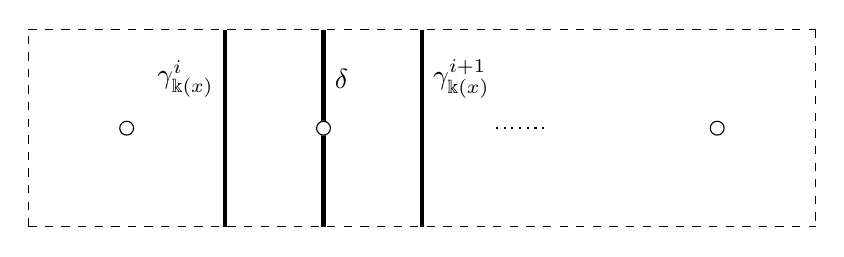
\begin{tikzpicture}[scale=2.5]
				% fundamental square
				% n= 4
				\draw[dashed] (0,0)--(4,0);
				\draw[dashed] (0,0)--(0,1);
				\draw[dashed] (0,1)--(4,1);
				\draw[dashed] (4,1)--(4,0);

				% white square

				\filldraw[white] (2+0.5,0.5) circle (0.275);

				\draw[dotted, thick] (2+0.5-0.125,0.5)--(2+0.5+0.125,0.5);

				% \Bbbk(x)
				\draw[line width=1.5, black] (1,0)--(1, 0.75) node[left]{$\gamma_{\Bbbk(x)}^i$};
				\draw[line width=1.5, black] (1,0.75)--(1,1);

				\draw[line width=1.5, black] (2,0)--(2, 0.75) node[right]{$\gamma_{\Bbbk(x)}^{i+1}$};
				\draw[line width=1.5, black] (2,0.75)--(2,1);

				\draw[line width=1.5, black] (1.5,0)--(1.5, 0.75) ;
				\draw[line width=1.5, black] (1.5,1)--(1.5,0.75) node[right]{$\delta$};

				\foreach \u in {0,1,3}
					{
						% marked points
						\filldraw[white] (\u+0.5,0.5) circle (1pt);
						\draw[black] (\u+0.5,0.5) circle (1pt);

					}
			\end{tikzpicture}
		\end{displaymath}
		\caption{}
	\end{figure}

\end{proposition}
\begin{thebibliography}{99}
	\bibitem[BD11]{BD11} Farb, Benson, and Dan Margalit, \textit{A Primer on Mapping Class Groups (PMS-49)} (Princeton, NJ, 2011; online edn, Princeton Scholarship Online, 19 Oct. 2017)
	\bibitem[Huy06]{Huy06} D. Huybrechts, \textit{Fourier-Mukai transforms in algebraic geometry}, Oxford Math. Monogr. (The
	Clarendon Press, Oxford Univ. Press, Oxford, 2006); http://dx.doi.org/10.1093/acprof:
	oso/9780199296866.001.0001.
	\bibitem[IU05]{IU05} A. Ishii and H. Uehara, \textit{Autoequivalences of derived categories on the minimal resolutions of An-singularities on surfaces}, J. Differential Geom. 71 (2005), no. 3, 385–435; http://projecteuclid.org/euclid.jdg/1143571989.
	\bibitem[Opp20]{Opp20} S. Opper, \textit{Spherical objects, transitivity and auto-equivalences of Kodaira cycles via gentle algebras
	},arXiv e-prints (2021), arXiv:2011.08288.
	\bibitem[Ueh15]{Ueh15} H. Uehara, \textit{Autoequivalences of derived categories of elliptic surfaces with non-zero Kodaira dimension},arXiv e-prints (2021), arXiv:1501.06657v2.
\end{thebibliography}
\end{document}